\makeatletter\let\ifGm@compatii\relax\makeatother
\RequirePackage{atbegshi}
\documentclass[final,hyperref={pdfpagemode=FullScreen},aspectratio=169,10pt]{beamer}

\usepackage[english]{babel}
\usepackage{lmodern,hyperref,amsmath,amssymb,pdftexcmds,listings,lstautogobble,tikz,ulem,xspace}
\usepackage{appendixnumberbeamer}
\usepackage[utf8]{luainputenc}
\usepackage[T1]{fontenc}
\usepackage{fontawesome5}
\usepackage{qrcode}
\usepackage[export]{adjustbox}
%\ttfamily\DeclareFontShape{T1}{lmtt}{m}{it}
%                          {<->sub*lmtt/m/sl}{}

%\usetheme{Pittsburgh}
%\usecolortheme{seahorse}
\usetheme{metropolis}
\metroset{sectionpage=progressbar} % or none
\metroset{numbering=counter} % or none, fraction
\metroset{progressbar=frametitle}
\setbeamercovered{transparent}

% Header and footer
\beamertemplatenavigationsymbolsempty
%\makeatletter
\setbeamertemplate{footline}
{
  \leavevmode%
  \hbox{%
  \begin{beamercolorbox}[wd=.333333\paperwidth,ht=2.25ex,dp=1ex,center]{author in head/foot}%
    \usebeamerfont{author in head/foot}\insertshorttitle{}
  \end{beamercolorbox}%
  \begin{beamercolorbox}[wd=.333333\paperwidth,ht=2.25ex,dp=1ex,center]{title in head/foot}%
    \usebeamerfont{title in head/foot}\insertshortdate{}
  \end{beamercolorbox}%
  \begin{beamercolorbox}[wd=.333333\paperwidth,ht=2.25ex,dp=1ex,right]{date in head/foot}%
    \usebeamerfont{date in head/foot}
    \insertframenumber{} / \inserttotalframenumber\hspace*{2ex}
  \end{beamercolorbox}}%
  \vskip0pt%
}
\makeatother
\setbeamerfont{footnote mark}{size=\tiny}
\setbeamerfont{footnote}{size=\tiny}

\newlength{\spaceheight}
\setlength{\spaceheight}{\textheight}
\addtolength{\spaceheight}{-\headheight}
\addtolength{\spaceheight}{-\headsep}

% Wide pages for large photos
\newcommand\Wider[2][3em]{%
\makebox[\linewidth][c]{%
  \begin{minipage}{\dimexpr\textwidth+#1\relax}
  \raggedright#2
  \end{minipage}%
  }%
}


% Colors and fonts
\definecolor{beamerbackgroundcolor}{RGB}{250,250,250}
\definecolor{rootbackground}{RGB}{49,97,151}
\definecolor{myyellow}{RGB}{242,226,149}
\definecolor{rootforeground}{HTML}{1ed4e5}
\definecolor{altalert}{HTML}{ae2012}
\definecolor{mygreen}{HTML}{c7f9cc}
\definecolor{myred}{HTML}{f8ad9d}
\setbeamercolor{block title}{fg=black,bg=red!30!black!30}
\setbeamercolor{block body}{fg=black,bg=beamerbackgroundcolor!96!black}
\setbeamercolor{block title alerted}{fg=red,bg=gray!40}
\setbeamercolor{block title example}{fg=black,bg=green!20}
\setbeamercolor{block body example}{fg=black,bg=green!5}
\setbeamercolor{block body alerted}{fg=black,bg=red!5}
\setbeamerfont{block title}{series=\bfseries}

\setbeamercolor{title}{fg=white}
\setbeamercolor{author}{fg=white}
\setbeamercolor{date}{fg=white}
\setbeamercolor{frametitle}{bg=rootbackground}
\setbeamercolor{section title}{fg=rootbackground} % Actually: link color
\setbeamercolor{author in head/foot}{bg=beamerbackgroundcolor, fg=rootbackground}
\setbeamercolor{title in head/foot}{bg=beamerbackgroundcolor, fg=rootbackground}
\setbeamercolor{date in head/foot}{bg=beamerbackgroundcolor, fg=rootbackground}


% Backup slides
\newcommand{\beginbackup}{
   \newcounter{framenumbervorappendix}
   \setcounter{framenumbervorappendix}{\value{framenumber}}
}
\newcommand{\backupend}{
   \addtocounter{framenumbervorappendix}{-\value{framenumber}}
   \addtocounter{framenumber}{\value{framenumbervorappendix}}
}


% Framed blocks
\makeatletter
\newcommand\beamerboxesframed[2][]{%
  \global\let\beamer@firstlineitemizeunskip=\relax%
  \vbox\bgroup%
  \setkeys{beamerboxes}{upper=block title,lower=block body,width=\textwidth}%
  \setkeys{beamerboxes}{#1}%
  {%
    \usebeamercolor{\bmb@lower}%
    \globalcolorstrue%
    \colorlet{lower.bg}{bg}%
  }%
  {%
    \usebeamercolor{\bmb@upper}%
    \globalcolorstrue%
    \colorlet{upper.bg}{bg}%
  }%
  %
  % Typeset head
  %
  \vskip4bp
  \setbox\bmb@box=\hbox{%
    \begin{minipage}[b]{\bmb@width}%
      \usebeamercolor[fg]{\bmb@upper}%
      #2%
    \end{minipage}}%
  \ifdim\wd\bmb@box=0pt%
    \setbox\bmb@box=\hbox{}%
    \ht\bmb@box=0pt%
    \bmb@prevheight=-4.5pt%
  \else%
    \wd\bmb@box=\bmb@width%
    \bmb@temp=\dp\bmb@box%
    \ifdim\bmb@temp<1.5pt%
      \bmb@temp=1.5pt%
    \fi%
    \setbox\bmb@box=\hbox{\raise\bmb@temp\hbox{\box\bmb@box}}%
    \dp\bmb@box=0pt%
    \bmb@prevheight=\ht\bmb@box%
  \fi%
  \bmb@temp=\bmb@width%
  \bmb@dima=\bmb@temp\advance\bmb@dima by2.2bp%
  \bmb@dimb=\bmb@temp\advance\bmb@dimb by4bp%
  \hbox{%
    \begin{pgfpicture}{0bp}{+-\ht\bmb@box}{0bp}{+-\ht\bmb@box}
      \ifdim\wd\bmb@box=0pt%
        \color{lower.bg}%
      \else%
        \color{upper.bg}%
      \fi%
      \pgfpathqmoveto{-4bp}{-1bp}
      \pgfpathqcurveto{-4bp}{1.2bp}{-2.2bp}{3bp}{0bp}{3bp}
      \pgfpathlineto{\pgfpoint{\bmb@temp}{3bp}}
      \pgfpathcurveto%
      {\pgfpoint{\bmb@dima}{3bp}}%
      {\pgfpoint{\bmb@dimb}{1.2bp}}%
      {\pgfpoint{\bmb@dimb}{-1bp}}%
      \bmb@dima=-\ht\bmb@box%
      \advance\bmb@dima by-2pt%
      \pgfpathlineto{\pgfpoint{\bmb@dimb}{\bmb@dima}}
      \pgfpathlineto{\pgfpoint{-4bp}{\bmb@dima}}
      \pgfpathclose
      \pgfsetstrokecolor{black}\pgfusepath{stroke, fill}
    \end{pgfpicture}%
    \copy\bmb@box%
  }%
  \nointerlineskip%
  \ifdim\wd\bmb@box=0pt
  \else
    \vskip2.4pt%
  \fi%
  \nointerlineskip%
  \setbox\bmb@colorbox=\hbox{{\pgfpicturetrue\pgfsetcolor{lower.bg}}}%
  \setbox\bmb@box=\hbox\bgroup\begin{minipage}[b]{\bmb@width}%
    \vskip2pt%
    \usebeamercolor[fg]{\bmb@lower}%
    \colorlet{beamerstructure}{upper.bg}%
    \colorlet{structure}{upper.bg}%
    %\color{.}%
}
\def\endbeamerboxesframed{%
  \end{minipage}\egroup%
  \wd\bmb@box=\bmb@width%
  \bmb@temp=\dp\bmb@box%
  \advance\bmb@temp by.5pt%
  \setbox\bmb@box=\hbox{\raise\bmb@temp\hbox{\box\bmb@box}}%
  \dp\bmb@box=0pt%
  \bmb@temp=\wd\bmb@box%
  \bmb@dima=\bmb@temp\advance\bmb@dima by2.2bp%
  \bmb@dimb=\bmb@temp\advance\bmb@dimb by4bp%
  \hbox{%
    \begin{pgfpicture}{0bp}{0bp}{0bp}{0bp}
      \unhbox\bmb@colorbox%
      \pgfpathmoveto{\pgfpoint{-4bp}{\ht\bmb@box}}
      \pgfpathlineto{\pgfpoint{-4bp}{1bp}}
      \pgfpathqcurveto{-4bp}{-1.2bp}{-2.2bp}{-3bp}{0bp}{-3bp}
      \pgfpathlineto{\pgfpoint{\the\bmb@temp}{-3bp}}
      \pgfpathcurveto%
      {\pgfpoint{\the\bmb@dima}{-3bp}}%
      {\pgfpoint{\the\bmb@dimb}{-1.2bp}}%
      {\pgfpoint{\the\bmb@dimb}{1bp}}%
      {
      \bmb@dima=\ht\bmb@box%
      \pgfpathlineto{\pgfpoint{\bmb@dimb}{\bmb@dima}}
      \pgfsetstrokecolor{black}\pgfusepath{stroke, fill}
      }
    \end{pgfpicture}%
    \box\bmb@box%
  }%
  \vskip2bp%
  \egroup% of \vbox\bgroup
}
\makeatother
\defbeamertemplateparent{blocks}[framed]{block begin,block end,%
  block alerted begin,block alerted end,%
  block example begin,block example end}[1][]
{[#1]}

\defbeamertemplate{block begin}{framed}[1][]
{
  \par\vskip\medskipamount%
  \begin{beamerboxesframed}[upper=block title,lower=block body,#1]%
    {\raggedright\usebeamerfont*{block title}\insertblocktitle}%
    \raggedright%
    \usebeamerfont{block body}%
}
\defbeamertemplate{block end}{framed}[1][]
{\end{beamerboxesframed}\vskip\smallskipamount}

\defbeamertemplate{block alerted begin}{framed}[1][]
{
  \par\vskip\medskipamount%
  \begin{beamerboxesframed}[upper=block title alerted,lower=block body alerted,#1]%
    {\raggedright\usebeamerfont*{block title alerted}\insertblocktitle}%
    \raggedright%
    \usebeamerfont{block body alerted}%
}%
\defbeamertemplate{block alerted end}{framed}[1][]
{\end{beamerboxesframed}\vskip\smallskipamount}

\defbeamertemplate{block example begin}{framed}[1][]
{
  \par\vskip\medskipamount%
  \begin{beamerboxesframed}[upper=block title example,lower=block body example,#1]
    {\raggedright\usebeamerfont*{block title example}\insertblocktitle}%
    \raggedright%
    \usebeamerfont{block body alerted}%
}%
\defbeamertemplate{block example end}{framed}[1][]
{\end{beamerboxesframed}\vskip\smallskipamount}

\setbeamertemplate{blocks}[framed]
% Use for normal blocks: \setbeamertemplate{blocks}[rounded][shadow=true]

\newenvironment<>{varblock}[2][\textwidth]{%
   \setlength{\textwidth}{#1}
   \begin{actionenv}#3%
     \def\insertblocktitle{#2}%
     \par%
     \usebeamertemplate{block begin}}
   {\par%
     \usebeamertemplate{block end}%
   \end{actionenv}}

\addtobeamertemplate{frametitle}{}{
\addvspace{-0.95cm}
\hfill
\includegraphics[height=0.75cm]{img/root-logo}
}

\setbeamercolor{section title}{fg=red}
\setbeamertemplate{blocks}[rounded][shadow=true]
\def\duration#1{\hfill[#1]}

\makeatletter
\let\@@TOC=\tableofcontents
\def\tableofcontents[#1]{\bgroup\parskip=0pt\@@TOC[#1]\egroup}
\makeatother

\AtBeginDocument{
  \setbeamertemplate{section in toc}[square]
  \setbeamertemplate{subsection in toc}{\hspace{1.3em}\rule[0.3ex]{4pt}{4pt}~\inserttocsubsection\par}
  \setbeamertemplate{itemize items}{\raisebox{.5ex}{\rule{.5ex}{.5ex}}}
  \setbeamercolor{alerted text}{fg=altalert}
}

\def\maketitle{%
    {\setbeamercolor{background canvas}{bg=rootbackground}
    \setbeamercolor{alerted text}{fg=rootforeground}
    \begin{frame}[plain,noframenumbering,label=titlepage]
        \centering
        \vspace{0.75cm}
\includegraphics[width=2cm]{img/root-splash.png}%
        \vspace{-1.5cm}\titlepage
    \end{frame}}}
\def\makeendpage{%
    {\setbeamercolor{background canvas}{bg=rootbackground}
    \setbeamercolor{alerted text}{fg=rootforeground}
    \begin{frame}[plain,noframenumbering,label=titlepage]
        \centering
        \vfill
        \tikz{
            \path node[opacity=.1] {
\includegraphics[width=7cm]{img/root-splash.png}}
                node[font={\fontsize{24}{24}\selectfont},white] {Thank you!};
        }
        \vfill
    \end{frame}}}

%\setsansfont[BoldFont=Fira Sans Regular,ItalicFont=Fira Sans Light Italic,Ligatures=NoCommon]{Fira Sans Light}
%\setmathfont{FiraSans-ThinItalic.ttf}

\def\linkbox#1#2{%
    \raisebox{-.5ex}{\tikz{\node[font=\footnotesize,myyellow!70!black!80,draw,rounded corners,fill=myyellow!70!white!20]{\blacktriangleright~\href{#1}{#2}};}}
}

\def\overlaynote#1{%
    \tikz[remember picture,overlay]{\node[fill=black!5,draw,rounded corners,text width=\textwidth,blur shadow] at (current page) {#1\vspace{1ex}};}
}

\makeatletter
\pgfdeclareshape{document}{
\inheritsavedanchors[from=rectangle] % this is nearly a rectangle
\inheritanchorborder[from=rectangle]
\inheritanchor[from=rectangle]{center}
\inheritanchor[from=rectangle]{north}
\inheritanchor[from=rectangle]{south}
\inheritanchor[from=rectangle]{west}
\inheritanchor[from=rectangle]{east}
% ... and possibly more
\backgroundpath{% this is new
% store lower right in xa/ya and upper right in xb/yb
\southwest \pgf@xa=\pgf@x \pgf@ya=\pgf@y
\northeast \pgf@xb=\pgf@x \pgf@yb=\pgf@y
% compute corner of ??flipped page??
\pgf@xc=\pgf@xb \advance\pgf@xc by-10pt % this should be a parameter
\pgf@yc=\pgf@yb \advance\pgf@yc by-10pt
% construct main path
\pgfpathmoveto{\pgfpoint{\pgf@xa}{\pgf@ya}}
\pgfpathlineto{\pgfpoint{\pgf@xa}{\pgf@yb}}
\pgfpathlineto{\pgfpoint{\pgf@xc}{\pgf@yb}}
\pgfpathlineto{\pgfpoint{\pgf@xb}{\pgf@yc}}
\pgfpathlineto{\pgfpoint{\pgf@xb}{\pgf@ya}}
\pgfpathclose
% add little corner
\pgfpathmoveto{\pgfpoint{\pgf@xc}{\pgf@yb}}
\pgfpathlineto{\pgfpoint{\pgf@xc}{\pgf@yc}}
\pgfpathlineto{\pgfpoint{\pgf@xb}{\pgf@yc}}
\pgfpathlineto{\pgfpoint{\pgf@xc}{\pgf@yc}}
}
}
\makeatother

\NewDocumentCommand\StickyNote{O{6cm}mO{6cm}}{%
\node[
document,
draw,
drop shadow={
  shadow xshift=2pt,
  shadow yshift=-4pt
},
inner xsep=7pt,
fill=myyellow,
xslant=-0.1,
yslant=0.1,
inner ysep=10pt
] {\parbox[t][#1][c]{#3}{#2}};
}

\NewDocumentCommand\StickyNotePi{O{6cm}mO{6cm}}{%
\node[
document,
draw,
fill=myyellow,
inner xsep=10pt,
xslant=-0.1,
yslant=0.1,
inner ysep=0pt,
text depth=\the\dimexpr#1+2.5ex\relax
] {\parbox[t][#1][c]{#3}{#2}};
}

\NewDocumentCommand\StickyNoteMinusPi{O{6cm}mO{6cm}}{%
\node[
document,
draw,
fill=myyellow,
inner xsep=10pt,
xslant=0.1,
yslant=-0.1,
inner ysep=0pt,
text depth=\the\dimexpr#1+2.5ex\relax
] {\parbox[t][#1][c]{#3}{#2}};
}


\definecolor{deprecated}{HTML}{E85D04}

\def\deprecated{\tikz\node[draw,color=deprecated,densely dotted,fill=deprecated!50!white!30,rounded corners,font=\fontsize{6}{6}\selectfont]{DEPRECATED};}

\def\clingPrompt{\textcolor{black!34}{[cling]\$ }}

\def\llvmURL{https://llvm.org/}
\def\clingURL{https://github.com/root-project/cling/}
\def\cppyyURL{https://cppyy.readthedocs.io/}
\def\libinteropURL{https://compiler-research.org/libinterop/}
\def\flamegraphURL{https://github.com/brendangregg/FlameGraph}

\hypersetup{final,
	        plainpages=false,
	        %hyperfootnotes=false,
	        colorlinks=true,
	        linkcolor=rootbackground,
	        urlcolor=black,
	        citecolor=rootbackground,
	        pdfpagemode=UseOutlines,
	        pdfstartview=FitH,
	        pdfborder={0 0 0}}

% ---- pgfplots
\usepackage{pgfplots}
\pgfplotsset{compat=1.18}

% ---- tikz
\usepackage{tikz}
\usetikzlibrary{fit,matrix,positioning,chains,arrows.meta,shapes.multipart,shapes.geometric,pgfplots.groupplots,graphs,graphdrawing,shadows.blur}
\usegdlibrary{trees}
\pgfdeclarelayer{background}\pgfsetlayers{background,main}

% ---- listings
\usepackage{listing,lstautogobble}
\definecolor{lstkeyword}{HTML}{01497c}
\definecolor{lststring}{HTML}{a4133c}
\definecolor{lstcomment}{HTML}{718355}
\definecolor{lsthl}{HTML}{ffd166}
\definecolor{lstinline}{HTML}{D62B53}
\lstset{
    escapechar=`,
    tabsize=3,
    breaklines=true,
    basicstyle={\ttfamily\scriptsize},
    keywordstyle={\color{lstkeyword}\bfseries},
    commentstyle={\color{lstcomment}},
    stringstyle={\color{lststring}},
}
\lstdefinestyle{c++}{
    language=c++,
    backgroundcolor=\color{black!6},
%    keywordstyle=[2]{\color{lstkeyword}\bfseries},
%    morekeywords=[2]{},
}
\lstdefinestyle{bash}{
    language=bash,
    backgroundcolor=\color{black!6},
}
\newsavebox\lstlistingIn
\newsavebox\lstlistingWrap
\newsavebox\lstlistingCodeGen

\def\lsthl#1{\raisebox{-.1ex}{\tikz\node[inner sep=0pt,fill=lsthl]{#1};}}
\def\inlineCode#1{\raisebox{-.7ex}{\tikz{\node[font={\footnotesize\ttfamily},rounded corners,color=lstinline,fill=black!6]{#1};}}}

\title{Interpreted C++: Is that a thing?}
\subtitle{A journey through LLVM/clang-based C++ JITting}
\author[Javier López-Gómez]{Javier López-Gómez for the ROOT team}
\date{\texttt{using std::cpp}, 2024-04-25}

\begin{document}
\maketitle
% ==== About me ====
\begin{frame}{About me}
  \begin{raggedleft}
    \tikz{\path node(pic) {
\includegraphics[width=.75in]{img/my-picture.png}}
      node(name) [right=0pt of pic,font={\bfseries},text width=2.5in] {\underline{Javier Lopez-Gomez}}
      node[below=0pt of name,text width=2.5in] {\small%
        \faGithub~\href{https://github.com/jalopezg-git}{jalopezg-git}\hfill
        \faGlobe~\href{https://jalopezg.dev/}{https://jalopezg.dev/}\\
        \faEnvelope~javier.lopez.gomez AT proton.me};}\\
  \end{raggedleft}

  \vfill
  Summary of the last 5+ years (compilers-wise)\ldots{}
  \begin{itemize}
  \item 2017--2020: PhD in Computer Science and Technology (ARCOS-UC3M)
    \begin{itemize}
    \item Prototype implementation of C++ contracts (clang)
    \item Research internship at CERN in 2019: Definition shadowing in cling
    \end{itemize}
    \medskip

  \item 2020--2023: Senior Fellow (SFT, CERN)
    \begin{itemize}
    \item More cling -- but also RNTuple and general contributions to the ROOT project
    \end{itemize}
    \medskip

  \item \textbf{2024--(currently): Senior Compiler Engineer (Zimperium, Inc.)}
    \begin{itemize}
    \item Software obfuscation that operates directly AArch64 binaries
    \end{itemize}
  \end{itemize}
\end{frame}


\begin{frame}{Contents}
  \tableofcontents[hidesubsections]
\end{frame}

% ==== Introduction ====
\section{Introduction}

\begin{frame}[fragile]{Spoiler: how does C++ interpretation look like?}
  \def\clingPrompt{\textcolor{black!34}{[cling]\$ }}
  You can do
  \begin{lstlisting}[style=c++]
`\clingPrompt` template <typename T>
  T f(T a, T b) {
    return a + b;
  }
`\clingPrompt` f(42, 6)
(int) 48
  \end{lstlisting}

  \pause
  And then
  \begin{lstlisting}[style=c++]
`\clingPrompt` std::string S{"Hello,"};
`\clingPrompt` f(S, std::string{" world!"})
(std::basic_string<char, std::char_traits<char>, std::allocator<char> >) "Hello, world!"
  \end{lstlisting}

  \pause
  But also the abomination below
  \begin{lstlisting}[style=c++]
`\clingPrompt` std::vector<int> f{1, 2, 3};
`\clingPrompt` f
(std::vector<int> &) { 1, 2, 3 }
  \end{lstlisting}
\end{frame}

\begin{frame}{Why bothering to interpret C++?}
  \begin{itemize}
  \item Many languages already offer a REPL (Read-Eval-Print-Loop) even if not designed to be interpreted, e.g. \texttt{C\#}
  \item It aids a lot while learning the language: try things out!
  \item Iterative / exploratory prototyping
  \item Write 'scripts' that make use of C/C++ libraries

  \item \ldots{}
  \end{itemize}
\end{frame}

\begin{frame}{Current state of affairs}
  \begin{itemize}
    \itemsep=1ex

  \item Cling is built on Clang and LLVM 13 (enabling support for C++20)
  \item CUDA support
  \item Allows loading an external library (\texttt{.so} / \texttt{.dll}) and get access to its symbols, e.g. call a function
  \item Debugging and profiling of JITed code
  \item Undo steps
  \item Protection against invalid memory accesses, e.g. dereferencing a pointer that points to unmapped memory
  \end{itemize}
\end{frame}

\begin{frame}[fragile]{Current state of affairs}
  But also some features that one would expect from an interpreter (even if that's not ISO C++)\ldots{}
  \vfill
  \begin{itemize}
    \itemsep=1ex

  \item Top-level statements

  \item Print the result of expression evaluation

  \item \texttt{auto} synthesizing, i.e. \inlineCode{foo = 42.0;} is equivalent to \inlineCode{auto foo = 42.0;}\\
    (if \inlineCode{foo} not declared before) \deprecated{}

  \item Support for redefining entities, e.g.
\begin{lstlisting}[style=C++]
int foo = 0;
std::string foo{"Hello!"};
\end{lstlisting}
  \end{itemize}
\end{frame}

% ==== Foundations ====
\section{Foundations}

\begin{frame}{LLVM}
  \begin{itemize}
    \itemsep=1ex

  \item %\includegraphics[height=\baselineskip]{img/llvm.png}
    LLVM and clang to the rescue!
    \begin{center}
      
\includegraphics[width=1in]{img/LLVMWyvernSmall.png}
    \end{center}

  \item LLVM gives all the infrastructure required to build a compiler
    \begin{itemize}
    \item Basic data structures, e.g. \texttt{llvm::SmallVector}, or \texttt{llvm::Twine}
    \item An intermediate representation (LLVM IR)
    \item Lowering to machine code for many targets: x86\_64, ARM7, AArch64, RISC-V, etc.
    \item Machine-dependent and machine-independent optimization passes
    \item Generation of debug information
    \end{itemize}
  \end{itemize}

  \only<2->{
    \begin{tikzpicture}[remember picture,overlay]
      \node[anchor=east,opacity=.9] at ($(current page.east)+(-.85in,-1in)$) {\tikz{
          \StickyNotePi[0.6in]{\footnotesize And more!  See \url{\llvmURL}.}[1.9in]%
      }};
    \end{tikzpicture}
  }

  \only<3->{
    \begin{tikzpicture}[remember picture,overlay]
      \node[draw,fill=white] at (current page.center) {\tikz[start chain=c going right,node distance=11pt,
  every node/.style={font=\scriptsize},
  every on chain/.style={join=by ->},
  rect/.style={draw,fill=white,text width=1in,align=center,minimum height=22pt,inner sep=1pt},
  container/.style={draw,densely dotted,top color=black!6,bottom color=white,rounded corners}]{

  \begin{scope}[every node/.append style=on chain]
    \path node(test_cpp) {test.cpp}
    % Frontend
    node(lexer)[rect] {Lexical analysis\\ (Lexer)}
    node(parser)[rect] {Syntactic analysis\\ (Parser)}
    node(sema)[rect] {Semantic analysis\\ (Sema)}
    node(IR)[rect] {Generate IR}
    % Backend
    node(optI)[continue chain=c going below,node distance=42pt,rect] {Arch-independent optimization}
    node(optD)[continue chain=c going left,node distance=11pt,rect] {Arch-dependent optimization}
    node(codegen)[rect] {Code generation}
    %
    node(test_0) {test.o};
  \end{scope}

  % Symbol tables and AST
  \draw[<->] (parser) -- ++(up:30pt) node(symtabs)[at end,anchor=south,label={right:Symbol tables}]{\tikz\foreach \i
    in {0pt,-2pt,-4pt} \node[inner sep=4pt,draw,fill=white,xshift=\i,yshift=\i]{};};
  \draw[<->] (sema) -- ++(up:30pt) node(ast)[at end,anchor=south,label={right:AST}]{\tikz\graph[tree layout,level distance=4pt,sibling distance=4pt,nodes={circle,inner sep=1.5pt,as=,fill=black}]{ a -- { b, c }};};

  % Draw fronend and backend rectangles
  \begin{pgfonlayer}{background}
    \path node(fe)[container,inner xsep=4pt,inner ysep=3pt,yshift=-3pt,fit={(lexer)(parser)(sema)(IR)(ast)}]{}
          node(be)[container,inner xsep=4pt,inner ysep=12pt,yshift=6pt,fit={(optI)(optD)(codegen)}]{};

    \foreach \i/\j in {fe/{Compiler frontend},be/{Compiler backend (LLVM)}}
      \node[font={\scriptsize\bfseries},above=0pt of \i.north west,anchor=north west]{\j};
  \end{pgfonlayer}

}
};
    \end{tikzpicture}
  }
\end{frame}

\begin{frame}[fragile]{LLVM IR}
  % == PART 1
  \begin{onlyenv}<1>
   \begin{itemize}
      \itemsep=1ex

    \item LLVM IR may have 3 different representations: \textbf{in-memory} structures, assembly-like \textbf{plain-text}, or \textbf{serialized} form
    \item Let's play a bit to build the LLVM IR for a simple function!
    \end{itemize}
  \end{onlyenv}

  % == PART 2
  \begin{onlyenv}<2->
    \begin{lstlisting}[style=c++]
LLVMContext C;
auto builder = std::make_unique<IRBuilder<>>(C);
auto M = std::make_unique<Module>("main", C);

auto i32 = builder->getInt32Ty();
auto funcTy = FunctionType::get(`\lsthl{i32, \{i32, i32\}}`, /*isVarArg=*/false);
auto func = Function::Create(funcTy, GlobalValue::LinkageTypes::ExternalLinkage, `\lsthl{"func"}`, *M);
auto BB = BasicBlock::Create(C, "entry", func);
builder->SetInsertPoint(BB);
auto addVal = builder->`\lsthl{CreateAdd}`(func->getArg(0), func->getArg(1));
builder->`\lsthl{CreateRet}`(addVal);
M->print(errs(), /*AAW=*/nullptr);
    \end{lstlisting}
  \end{onlyenv}

  \begin{onlyenv}<3->
    \begin{tikzpicture}[remember picture,overlay]
      \node[draw,fill=white,font={\ttfamily\footnotesize}] at ($(current page.east)+(-2in,0pt)$) {
            \begin{minipage}{2.5in}
; ModuleID = 'main'\\
source\_filename = "main"\\
\\
{\bfseries define i32} \@func({\bfseries i32} \%0, {\bfseries i32} \%1) \{\\
entry:\\
\rule{20pt}{0pt}\%2 = {\bfseries add i32} \%0, \%1\\
\rule{20pt}{0pt}{\bfseries ret i32} \%2\\
\}\\
            \end{minipage}
      };
    \end{tikzpicture}
  \end{onlyenv}

\end{frame}

\begin{frame}[fragile]{LLVM JIT / ORC}
  LLVM can also JIT IR to current target's machine code\ldots{}%
  \footnote{Full example: \url{https://github.com/jalopezg-git/slides-using_stdcpp_2014/blob/master/code/llvm-ir.cpp}}

  \vfill
  \begin{lstlisting}[style=c++]
int main(int argc, char *argv[]) {
  using namespace llvm;
  InitializeNativeTarget();
  InitializeNativeTargetAsmPrinter();

  /* CREATE IR AS IN PREVIOUS SLIDE */
  
  auto EE = EngineBuilder(std::move(M)).setEngineKind(llvm::EngineKind::JIT).create();

  using FuncPtr_t = uint32_t (*)(uint32_t, uint32_t);
  auto pFunc = (FuncPtr_t)EE->getFunctionAddress("func");
  auto ret = `\lsthl{pFunc(42, 7)}`;
  errs() << "\nfunc() returned " << ret << "\n";

  return 0;
}
  \end{lstlisting}

  \only<2->{
    \begin{tikzpicture}[remember picture,overlay]
      \node[anchor=east,opacity=.9] at ($(current page.east)+(-.85in,-1in)$) {\tikz{\StickyNotePi[0.6in]{
            {\ttfamily func() returned 49}
          }[1.9in]%
      }};
    \end{tikzpicture}
  }
\end{frame}

\begin{frame}[fragile]{Clang as a library}
  % == PART 1
  \begin{onlyenv}<1>
    \begin{itemize}
      \itemsep=1ex

    \item Clang is basically a frontend that parses C / C++ / ObjectiveC and generates LLVM IR, i.e.
      \begin{itemize}
      \item It does lexical / gramatical /  semantic analysis on the source code + builds an AST
      \item LLVM takes over from there
      \end{itemize}

    \item E.g., the simple code\ldots{}
      \lstinputlisting[style=c++]{code/puts-simple.c}
    \end{itemize}
  \end{onlyenv}

  % == PART 2
  \begin{onlyenv}<2>
    \lstinputlisting[style=c++]{code/puts-simple.c}
    \vfill

    Has AST representation\footnote{Get this with \texttt{clang -c -Xclang -ast-dump -o /dev/stdout input.c}}
    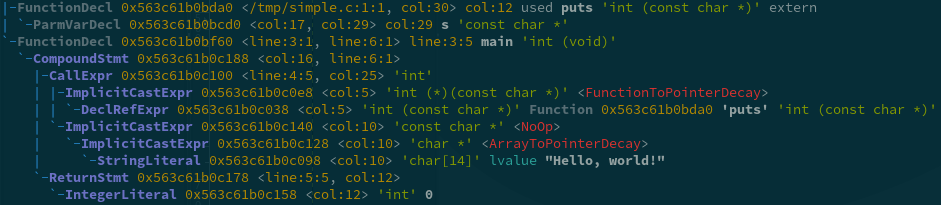
\includegraphics[width=\textwidth]{img/clang-ast.png}
  \end{onlyenv}

  % == PART 3
  \begin{onlyenv}<3>
    \lstinputlisting[style=c++]{code/puts-simple.c}
    \vfill

    And LLVM IR representation\footnote{Get this with \texttt{clang -S -emit-llvm -o /dev/stdout input.c}}
    \begin{lstlisting}[language=llvm,basicstyle={\ttfamily\fontsize{6.5}{6.5}\selectfont}]
; ModuleID = '/tmp/simple.c'
source_filename = "/tmp/simple.c"
target datalayout = "e-m:e-p270:32:32-p271:32:32-p272:64:64-i64:64-f80:128-n8:16:32:64-S128"
target triple = "x86_64-pc-linux-gnu"

@.str = private unnamed_addr constant [14 x i8] c"Hello, world!\00", align 1

; Function Attrs: nofree nounwind sspstrong uwtable
define dso_local i32 @main() local_unnamed_addr #0 {
  %1 = tail call i32 @puts(ptr noundef nonnull dereferenceable(1) @.str)
  ret i32 0
}

; Function Attrs: nofree nounwind
declare noundef i32 @puts(ptr nocapture noundef readonly) local_unnamed_addr #1
    \end{lstlisting}
  \end{onlyenv}
\end{frame}

\begin{frame}{Clang as a library}
  \begin{itemize}
    \itemsep=1ex

  \item And it offers libTooling, libclang-cpp, and libclang!

  \item Meaning we can mostly reuse this%
    \footnote{Modulo some patches required to clang.}%
    and only write a layer on top that does ``impedance matching'' between ISO and interpreted C++
  \end{itemize}
\end{frame}

% ==== The cling C++ interpreter ====
\section{The cling C++ interpreter}

\begin{frame}[fragile]{Cling's pipeline}
  \begin{lrbox}{\lstlistingIn}
   \begin{lstlisting}[style=c++,backgroundcolor={}]
`\clingPrompt` puts("Hello, world!");
   \end{lstlisting}
\end{lrbox}
\begin{lrbox}{\lstlistingWrap}
   \begin{lstlisting}[style=c++,backgroundcolor={}]
void __cling_Un1Qu30(void *) {
    puts("Hello, world!");
}
   \end{lstlisting}
\end{lrbox}
\begin{lrbox}{\lstlistingCodeGen}
  \begin{lstlisting}[language=llvm]
@.str = private unnamed_addr constant [14 x i8] c"Hello, world!\00", align 1

; Function Attrs: nofree nounwind sspstrong uwtable
define dso_local void @__cling_Un1Qu30(ptr nocapture noundef readnone %0) local_unnamed_addr {
  %2 = tail call i32 @puts(ptr noundef nonnull dereferenceable(1) @.str)
  ret void
}
  \end{lstlisting}
\end{lrbox}

\tikz[start chain=c going below,node distance=15pt,
  every node/.style={font=\scriptsize},
  every on chain/.style={join=by ->},
  rect/.style={top color=white,bottom color=teal!50!black!20,draw=teal!50!black!50,text width=1.75in,align=center,minimum height=20pt,inner sep=1pt,rounded corners},
  expl line/.style={dotted,black!25,->},
  expl/.style={draw,black,densely dotted,fill=white,font={\ttfamily\scriptsize},text width=2.5in}]{

  \def\ASTpre{\tikz\graph[tree layout,level distance=4pt,sibling distance=4pt,nodes={circle,inner sep=1.5pt,as=,fill=black}]{ a -- { b, c }};}
  \def\ASTpost{\tikz\graph[tree layout,level distance=4pt,sibling distance=4pt,nodes={circle,inner sep=1.5pt,as=,fill=black}]{ a -- { b -- { c, d }, e -- f }};}
  \def\sepRule{\rule{27pt}{0pt}}

  \begin{scope}[every node/.append style=on chain]
    \path node(in) {User input}
    node(wrap)[rect] {Wrap top-level statements}
    node(parse)[rect] {Parse (clang)}
    node(transform)[rect] {AST transformers}
    node(codegen)[rect] {Code generation}
    node(callwrapper)[rect] {Call wrapper function\\(if any)};
  \end{scope}

  % Step-by-step explanation
  \draw<1->[expl line] (in) -- ++(right:2in) node(in_expl)[at end,anchor=west,expl]{%
    \usebox{\lstlistingIn}
  };
  \draw<2->[expl line] (wrap) -- ++(right:2in) node(wrap_expl)[at end,anchor=west,expl]{%
    \usebox{\lstlistingWrap}
  };
  \draw<3->[expl line] (parse) -- ++(right:2in) node(parse_expl)[at end,anchor=west,expl]{%
    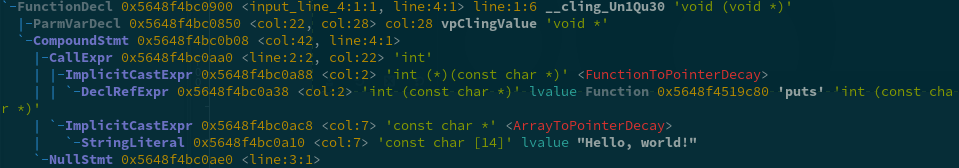
\includegraphics[width=\textwidth]{img/clang-ast-expl.png}
  };
  \draw<4->[expl line] (transform) -- ++(right:2in) node(transform_expl)[at end,anchor=west,black,solid]{%
    \ASTpre \sepRule $\rightarrow$ \sepRule \ASTpost
  };
  \draw<5->[expl line] (codegen) -- ++(right:2in) node(codegen_expl)[at end,anchor=west,expl]{%
    \resizebox{\textwidth}{!}{\usebox{\lstlistingCodeGen}}
  };
  \draw<6->[expl line] (callwrapper) -- ++(right:2in) node(callwrapper_expl)[at end,anchor=west,expl]{%
    [If $\exists$ top-level statement, get a pointer to the wrapper function and do indirect call]
  };

}


  \only<7->{
    \begin{tikzpicture}[remember picture,overlay]
      \node[anchor=east,opacity=.9] at ($(current page.east)+(-.85in,-.8in)$) {\tikz{
          \StickyNotePi[1.2in]{
            \begin{itemize}
            \item Deferred (implicit) template instantiations \textbf{must} be emitted; we do that by forcing a end-of-TU event!
            \item CodeGen: also involves linking (external symbol resolution, etc.)
            \end{itemize}
          }[3in]%
      }};
    \end{tikzpicture}
  }
\end{frame}

\begin{frame}[fragile]{Transactions}
  \begin{itemize}
    \itemsep=1ex

  \item AST is built incrementally

  \item \textbf{Transaction:} declarations that were parsed and emitted in a single step
    \begin{itemize}
    \item User-provided declarations
    \item Implicit template instatiations
    \item Deserialized declarations from a C++ module
    \end{itemize}

  \item And allows undoing it.  That's useful, e.g. after a failed parse
%    \begin{lstlisting}[style=c++]
%`\clingPrompt` auto p = std::make_unique<std::string>("Hi there!");
%`\clingPrompt` `\lsthl{p.size()}`
%  error: no member named 'size' in 'std::unique_ptr<std::basic_string<char>, std::default_delete<std::basic_string<char> > >'; did you mean to use '->' instead of '.'?
%  p.size()
%   ^
%    \end{lstlisting}
  \end{itemize}
\end{frame}

\begin{frame}[fragile]{Extensions}
  \begin{itemize}
    \itemsep=1ex

  \item Most extensions are implemented as an AST transformer
  \item Currently, there is support for
    \begin{itemize}
    \item \inlineCode{auto} synthesizing, e.g. \inlineCode{foobar = 42.0f;}
      \pause

    \item Protection against invalid pointer deferencing, e.g.
      \begin{lstlisting}[style=c++]
`\clingPrompt` *((int *)0xff00ff00) = 0;
Error in <HandleInterpreterException>: Trying to access a pointer that points to an invalid memory address.
Execution of your code was aborted.
ROOT_prompt_6:1:2: `\alert{warning:}` invalid memory pointer passed to a callee:
*((int *)0xff00ff00) = 0;
 ^~~~~~~~~~~~~~~~~~~
      \end{lstlisting}
      \pause

    \item Shadowing of definitions
      \begin{lstlisting}[style=c++]
`\clingPrompt` int foobar = 0;
`\clingPrompt` std::string foobar() { return "A string!"; }
      \end{lstlisting}
      \pause

    \item Printing / capturing the value of an expression
      \begin{lstlisting}[style=c++]
`\clingPrompt` foobar()
(std::string) "A string!"
      \end{lstlisting}
    \end{itemize}
  \end{itemize}
\end{frame}

\begin{frame}[fragile]{Debugging / Profiling of JIT'ed code}
  Cling also allows debugging JITed code and offers integration with Linux's \texttt{perf}, e.g.
  \vfill

  \begin{itemize}
  \item A breakpoint on interpreted code can be set and step-into after each statement

  \item It can generate a symbol file for \texttt{perf} -- Can be used together with Flamegraph%
    \footnote{Flamegraph: \url{\flamegraphURL}}!
  \end{itemize}
\end{frame}

\begin{frame}{The future of cling: \protect\texttt{clang-repl}}
  \begin{itemize}
    \itemsep=1ex

  \item Cling proved to perform okay in the context of the larger ROOT project at CERN

  \item Let's upstream the foundations of it back to the LLVM community so that
    \begin{itemize}
    \item The whole community can benefit from it
    \item Maintenance is easier in the long term
    \end{itemize}

  \item \texttt{clang-repl}: already in recent versions of LLVM --- \alert{Thanks, Vassil!}

  \item Slightly different to the design of cling, e.g. modeling of top-level statements is much more rubust
  \end{itemize}
\end{frame}

% ==== Closing words ====
\section{Closing words}

\begin{frame}{Closing words}
  \begin{block}{Key ideas to take home}
    \begin{itemize}
    \item Cling enables incremental C++ compilation and JITting
      \begin{itemize}
      \item It would not be possible without the solid framework provided by LLVM and clang
      \end{itemize}

    \item Convenient integration with Jupyter notebook via \texttt{xeus-cling}
    \item Try it!
    \end{itemize}
  \end{block}
  \vfill
  \begin{block}{For the curious}
    \begin{itemize}
    \item cppyy / libinterop provide interoperability with other languages
      \begin{itemize}
      \item Enabling crazy things such as injecting the C++ definition of a type \inlineCode{T} and creating an object of type \inlineCode{T} from Python

      \item Or even crazier: on-the-fly template instantiation, e.g. a \inlineCode{std::vector$<T>$}%
        \footnote{\cppyyURL}%
        \footnote{\libinteropURL}
      \end{itemize}
    \end{itemize}
  \end{block}
\end{frame}

\begin{frame}{How can I get it?}
  \begin{center}
    \qrcode[height=1in]{\clingURL}\\[1ex]
    \url{\clingURL}
  \end{center}

  \begin{itemize}
  \item If you have `llvm` installed locally, try \texttt{clang-repl}
  \end{itemize}
\end{frame}


\makeendpage
% ==== APPENDIX ====

\appendix
\end{document}
